\chapter{Multi-Party Computation}

\section{Introduction}
Multi-Party Computation (MPC), also known as Secure Function Evaluation, allows two or more parties
to correctly compute a function of their private inputs without exposure, i.e., without
the input of one party being revealed to the other parties.\\
A generic function \textit{f} receives as input a set $A = \{a_1,a_2,\dots,a_n\}$
of arguments, where $a_i$ is the input of the i-th party, and $1\leq i\leq n$, and outputs a value \textit{z}, which represents the result
of the joint computation of \textit{f}, as shown in Figure \ref{fig:mpcscheme}.\\
The output of \textit{f} is given by the following expression,
\begin{equation}\label{eq:mpc}
z = f(a_1,a_2,\dots,a_n)
\end{equation}

\renewcommand{\figurename}{Figure}
\begin{figure}[H]
\centering
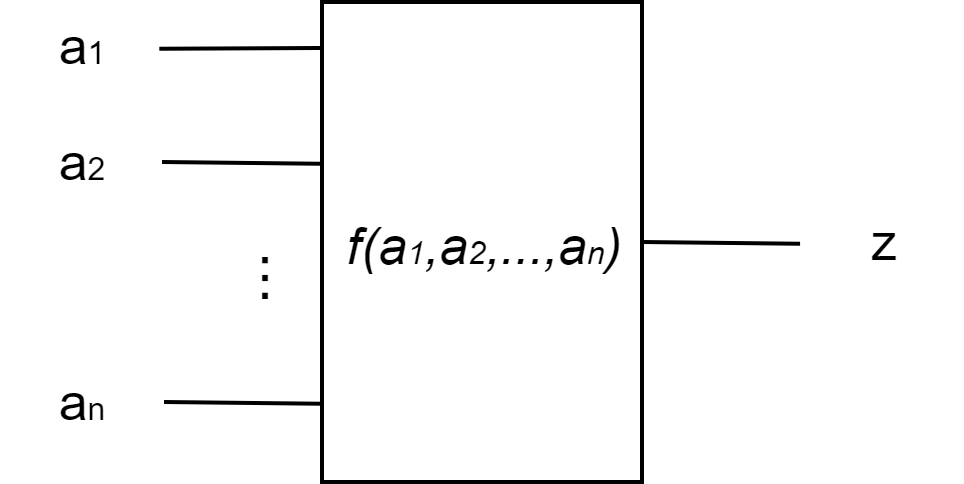
\includegraphics[width=.45\linewidth]{./figures/mpc/mpc_scheme}
\caption{Multi-Party Computation Diagram}
\label{fig:mpcscheme}
\end{figure}
\pagebreak

\section{Two-Party Computation}
Two-Party Computation (2PC) is a specific case of MPC, where a generic function \textit{f} receives as input a set $A = \{a,b\}$
of arguments, where \textit{a} is the input from the first party and \textit{b} is the input from the second,
and outputs a value \textit{c}, as shown in Figure \ref{fig:tpcscheme}.\\
The output of \textit{f} is given by the following expression,
\begin{equation}\label{eq:tpc}
c = f(a,b)
\end{equation}

An example of a 2PC problem, is \textbf{Yao's Millionaires' Problem}, in which 2 millionaires, Alice and Bob, are
interested in knowing which one of them is richer without revealing their wealth. The goal of this problem is to solve
the inequality $a\geq b$, where $a$ is Alice's input and $b$ is Bob's input, without revealing the values
of $a$ and $b$.

\renewcommand{\figurename}{Figure}
\begin{figure}[H]
\centering
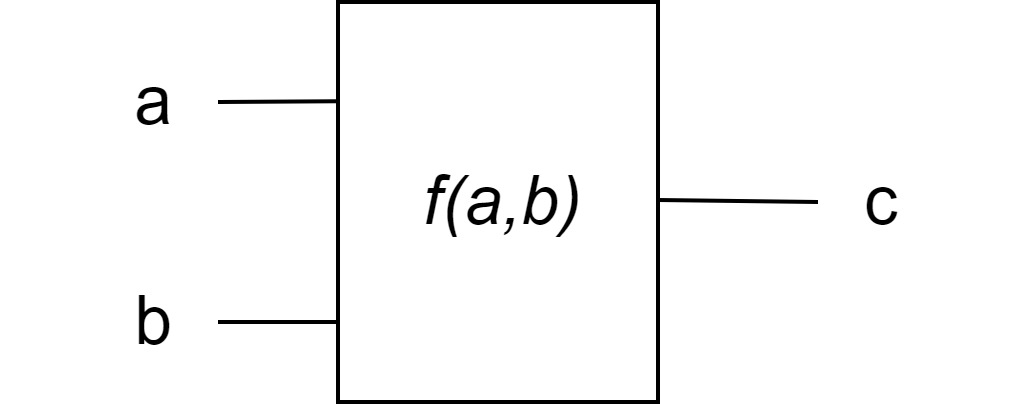
\includegraphics[width=.4\linewidth]{./figures/mpc/two_party_computation_scheme}
\caption{Two-Party Computation Diagram}
\label{fig:tpcscheme}
\end{figure}

\section{Oblivious Transfer}
Oblivious Transfer (OT) is a protocol that allows the sender to transfer one piece of information
to a receiver, but remains oblivious as to what piece has been transferred.\\
For example, consider two parties, Alice and Bob, where Alice has a set $M = \{m_0,m_1\}$ of messages
and Bob wants to obtain one of those messages, but won't reveal which one. By OT, Bob is able to
receive the message he wanted from Alice without Alice knowing which one she sent to Bob.

\renewcommand{\figurename}{Figure}
\begin{figure}[H]
\centering
\includegraphics[width=.4\linewidth]{./figures/mpc/OT}
\caption{Oblivious Transfer Diagram}
\label{fig:otscheme}
\end{figure}

\section{Garbled Circuit Protocol}
Introduced in 1986 by Andrew Yao, the Garbled Circuit protocol (GC) addresses the case
of Two-Party Computation (2PC), without the presence of a trusted third party.\\
GC allows a secure evaluation of a function given as a Boolean circuit that is represented as a series of logic gates.
The circuit is known to both parties.\\

\section{Hardware Description Languages}
Contrary to Programming Languages such as C or C++, which are used to specify a set of instructions to a computer, Hardware Description Languages (HDL) are computer languages used to describe the structure and behavior of digital logic circuits. They allow for the synthesis of HDL description code into a netlist (specification of physical eletronic components, such as AND gates or NOT gates, and how they are connected together).

\section{TinyGarble}
TinyGarble is a GC framework that takes advantage of powerful logic synthesis techniques, provided by both HDL synthesis tools
and TinyGarble's custom libraries, in order improve the overall efficiency of the GC protocol.\\
It it possible to describe the circuit using High-Level Programming Languages (HLPL) such as C, although High-Level Synthesis (HLS) is required. HLS is performed by High-Level Synthesis tools, such as SPARK for the C language.

\renewcommand{\figurename}{Figure}
\begin{figure}[H]
\centering
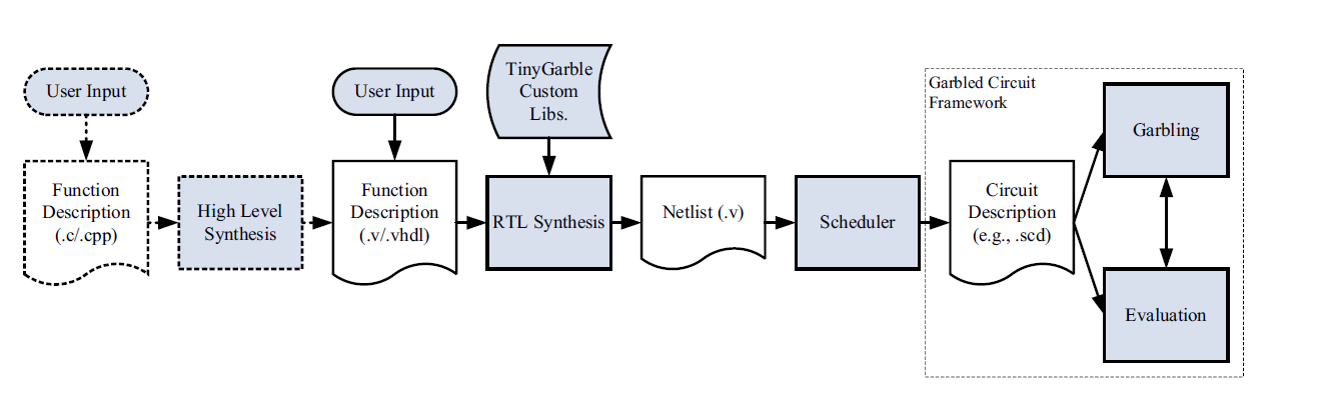
\includegraphics[width=.9\linewidth]{./figures/mpc/tinygarble_flow_diagram}
\caption{TinyGarble Flow Diagram}
\label{fig:tgdiagram}
\end{figure}

\section{ARM2GC}
Although circuit description in HLPL is possible, it is not very efficient when compared to HDL circuit description. ARM2GC addresses this problem, significantly improving the performance of garbled circuits described in HLPL.\\
In the case of 2PC, ARM2GC's approach to GC is based on the ARM processor architecture and consists in providing a public parameter to function \textit{f}, so that its output would be given by the following expression,
\begin{equation}\label{eq:arm2gc}
z = f(a,b,p)
\end{equation}
, where $p$ represents a public parameter, known to both parties.\\
In ARM2GC the Boolean circuit required to perform GC is that of a processor to which the compiled binary of the function is given as a public input ($p$\textit{ = compiled binary of the function}). This optimization is performed by the SkipGate algorithm.

%\bibliography{./chapter/mpcomputation} 